% Report/chapters/ff.tex

The FEniCS Project is a collaborative project for the development of innovative concepts and tools for automated scientific computing, with a particular focus on automated solution of differential equations by finite element methods. 
FEniCS has an extensive list of features for automated, efficient solution of differential equations, including automated solution of variational problems, automated error control and adaptivity, a comprehensive library of finite elements, high performance linear algebra and many more.

\smallskip
\noindent This chapter discusses how to solve a Boundary Value Problem, in particular 2D problems using FreeFEM++.

\section{Model Problem}
Consider the following model problem,
\begin{eqnarray}
	-\Delta u &=& f, \quad \text{in} \ \Omega \\
	u &=& z \quad \text{on} \ \Gamma_1\\
	\frac{\partial u}{\partial n}  &=& \nabla u . n = 0 \quad \text{on} \ \Gamma_2
\end{eqnarray}

The FEniCS code that solves the problem is given below.

\lstset{language = python}
\begin{lstlisting}
	-Laplace(u) = f on the unit square.
	u = u0 on the boundary.
	u0 = u = 1 + x^2 + 2y^2, f = -6.
	
	from dolfin import *
	mesh = UnitSquare(6, 4)
	V = FunctionSpace(mesh, 'Lagrange', 1)
	
	u0 = Expression('1 + x[0]*x[0] + 2*x[1]*x[1]')
	
	def u0_boundary(x, on_boundary):
	return on_boundary
	
	bc = DirichletBC(V, u0, u0_boundary)
	
	u = TrialFunction(V)
	v = TestFunction(V)
	f = Constant(-6.0)
	a = inner(nabla_grad(u), nabla_grad(v))*dx
	L = f*v*dx
	
	u = Function(V)
	solve(a == L, u, bc)
	
	plot(u)
	plot(mesh)
	
	interactive()
\end{lstlisting}

Let us first look at some important commands and syntax that are necessary to understand further problems.
\begin{lstlisting}
	from dolfin import *
\end{lstlisting}
This line imports the key classes UnitSquare, FunctionSpace, Function, and so forth, from the DOLFIN library. All FEniCS programs for solving PDEs by the finite element method normally start with this line. DOLFIN is a software library with efficient and convenient C++ classes for finite element computing, and dolfin is a Python package providing access to this C++ library from Python programs.

\begin{lstlisting}
	mesh = UnitSquare(6, 4)
\end{lstlisting}
The UnitSquare command defines a uniform finite element mesh over the unit square. The mesh consists of cells, which are triangles with straight sides. The parameters 6 and 4 tell that the square is first divided into 6×4 rectangles, and then each rectangle is divided into two triangles.
Other types of mesh generation will be discussed in the later part of this chapter.
\begin{lstlisting}
	V = FunctionSpace(mesh, 'Lagrange', 1)
\end{lstlisting}
The functionspace command defines a function space V with 3 arguments. The first argument is the mesh. The second argument reflects the type of element, while the third argument is the degree of the basis functions on the element.

\begin{figure}[h]
	\center
	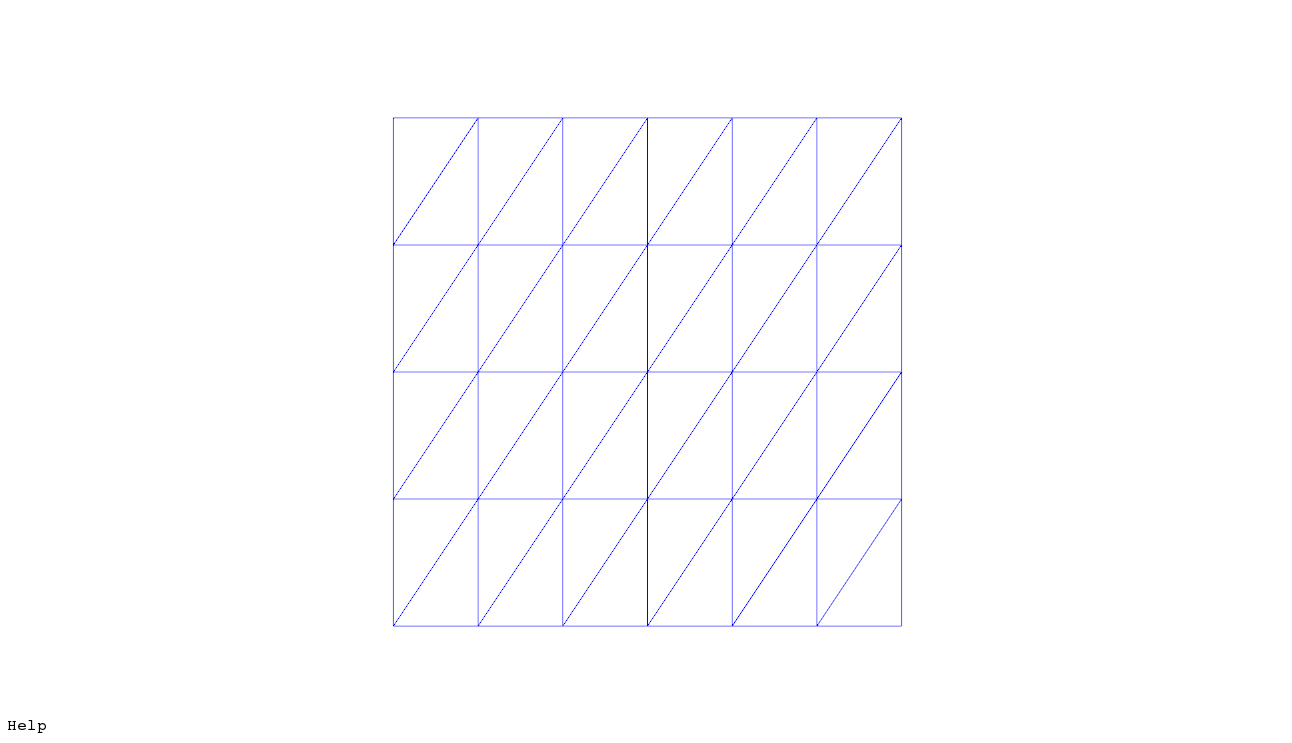
\includegraphics[scale = 0.25]{images/mesh.png}
	\caption{FEniCS Mesh}
\end{figure}

\begin{lstlisting}
	u = TrialFunction(V)
	v = TestFunction(V)
\end{lstlisting}
These commands define the finite dimensional trial and test spaces.
\begin{lstlisting}
	bc = DirichletBC(V, u0, u0_boundary)
\end{lstlisting}
The next step is to specify the boundary condition on the boundary.
\begin{lstlisting}
	f = Constant(-6.0)
\end{lstlisting}
When \textbf{f} is constant over the domain, \textbf{f} can be more efficiently represented as a Constant object.

We input the weak form of the problem 
\begin{eqnarray}
	 \int_{\Omega} \nabla u_h. \nabla v_h \ d\Omega - \int_{\Omega} f v_h \ d\Omega = 0
\end{eqnarray}
with the boundary condtions. The \textbf{solve} command solves the problem yielding $u_h$. 
\begin{lstlisting}
	a = inner(nabla_grad(u), nabla_grad(v))*dx
	L = f*v*dx
	u = Function(V)
	solve(a == L, u, bc)
\end{lstlisting}
Note that we first defined the variable $u$ as a TrialFunction and used it to represent the unknown in the form $a$. Thereafter, we redefined $u$ to be a Function object representing the solution, i.e., the computed finite element function $u$.
\begin{lstlisting}
	plot(u)
	plot(mesh)
	interactive()
\end{lstlisting}
This is the simplest way of quickly looking at $u$ and the mesh. The interactive() call is necessary for the plot to remain on the screen.

\pagebreak

\section{Meshing in Fenics}
In this section we will discuss a couple of standard mesh generation techniques.
\subsection{Built-in Mesh generation tools}
DOLFIN has a few tools for creating various types of meshes over domains with simple shape: \textbf{UnitInterval, UnitSquare, UnitCube, Interval, Rectangle, Box, UnitCircle, and UnitSphere}.
\begin{lstlisting}
	# 1D domains
	mesh = UnitInterval(20)     # 20 cells, 21 vertices
	mesh = Interval(20, -1, 1)  # domain [-1,1]

	# 2D domains (6x10 divisions, 120 cells, 77 vertices)
	mesh = UnitSquare(6, 10)  # 'right' diagonal is default
	# The diagonals can be right, left or crossed
	mesh = UnitSquare(6, 10, 'left')
	mesh = UnitSquare(6, 10, 'crossed')

	# Domain [0,3]x[0,2] with 6x10 divisions and left diagonals
	mesh = Rectangle(0, 0, 3, 2, 6, 10, 'left')

	# 6x10x5 boxes in the unit cube, each box gets 6 tetrahedra:
	mesh = UnitCube(6, 10, 5)

	# Domain [-1,1]x[-1,0]x[-1,2] with 6x10x5 divisions
	mesh = Box(-1, -1, -1, 1, 0, 2, 6, 10, 5)

	# 10 divisions in radial directions
	mesh = UnitCircle(10)
	mesh = UnitSphere(10)
\end{lstlisting}

\subsection{Other techniques}

Other standard techniques for importing/generating meshes into FEniCS are reading \textbf{.XML or .OFF} files, using the Mesheditor, using a few \textbf{CGAL} functions or using \textbf{dolfin-convert}.

\noindent XML and OFF files are formats which are useful for saving and communicating meshes, not for generating them. \textbf{CGAL} stands for Computational Geometry Algorithms Library. Some of the few commands in \textbf{CGAL} are \textbf{CircleMesh, EllipseMesh, SphereMesh, EllipsoidMesh, PolyhedralMeshGenerator, Add ,Subtract }etc

\pagebreak

\section{Linear Numerical examples}

\begin{lstlisting}
	-Laplace(u) = f on the unit square.
	u = u0 on the boundary.
	u0 = 1 + x^2 + 2y^2, f = -6.
\end{lstlisting}
\begin{figure}[h]
	\center
	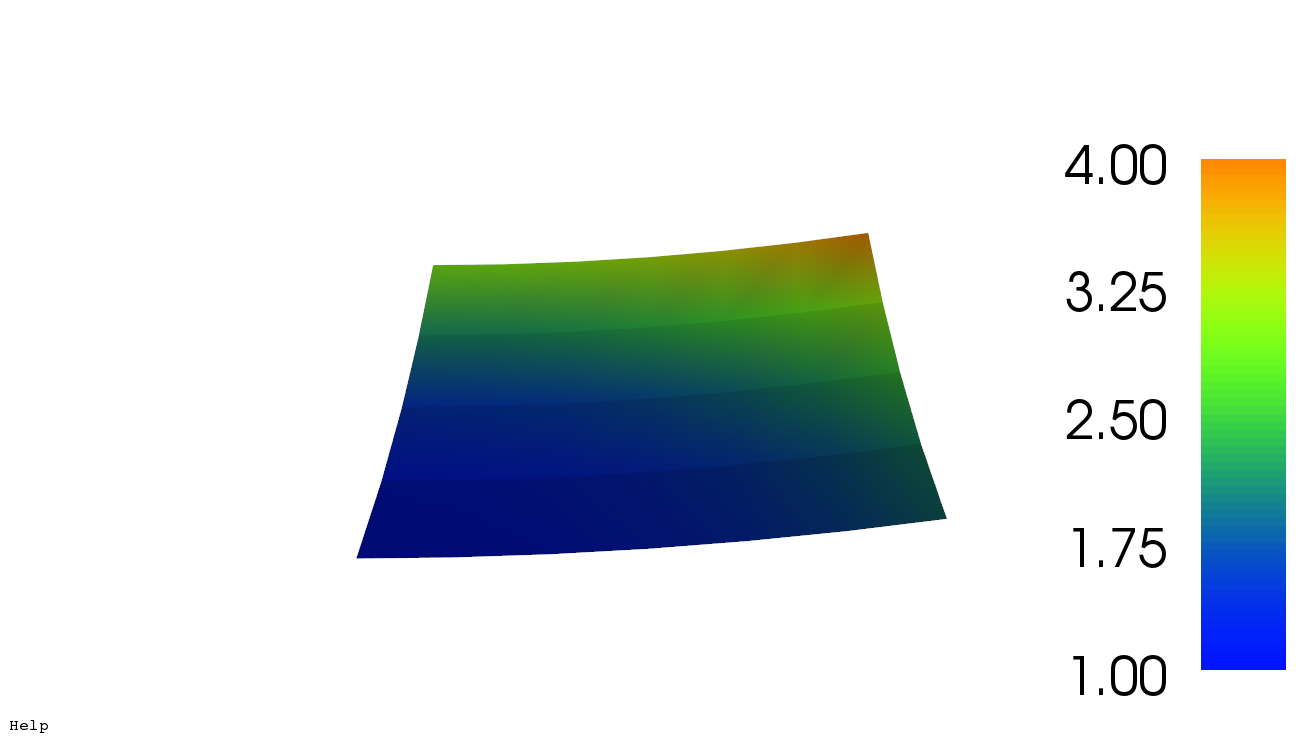
\includegraphics[scale = 0.25]{images/dirichlet.png}
	\caption{FEniCS Solution}
\end{figure}

Order of convergence data for Linear largrange element
\begin{lstlisting}
	Error norm based on infinity norm (of dofs)
	h=1.25E-01 E=3.75E-02 r=1.88
	h=6.25E-02 E=9.57E-03 r=1.97
	h=3.12E-02 E=2.41E-03 r=1.99
	h=1.56E-02 E=6.02E-04 r=2.00
	h=7.81E-03 E=1.51E-04 r=2.00
	h=3.79E-03 E=3.54E-05 r=2.00
\end{lstlisting}
\pagebreak
\noindent \textbf{Dirichlet Neumann Problem}
\begin{lstlisting}
	- div grad u(x, y) = f(x, y)
	on the unit square with source f given by
	f(x, y) = 10*exp(-((x - 0.5)^2 + (y - 0.5)^2) / 0.02)
	and boundary conditions given by
	u(x, y) = 0        for x = 0 or x = 1
	du/dn(x, y) = sin(5*x) for y = 0 or y = 1
\end{lstlisting}
\begin{figure}[h]
	\center
	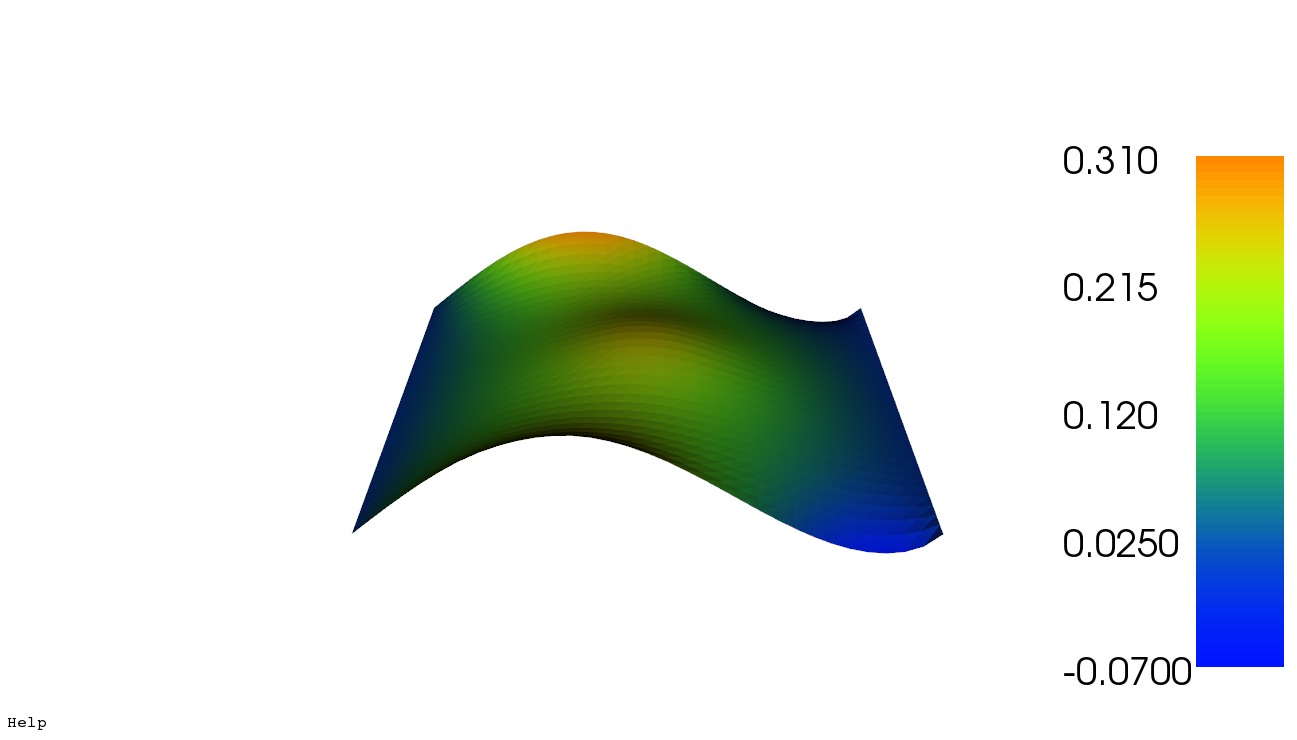
\includegraphics[scale = 0.25]{images/dn.png}
	\caption{FEniCS Solution}
\end{figure}
\noindent The order of convergence data for cubic Lagrange element
\begin{lstlisting}
	Error norm based on infinity norm (of dofs)
	h=5.00E-02 E=7.36E-06 r=3.97588
	h=2.50E-02 E=4.62E-07 r=3.99406
	h=1.25E-02 E=2.89E-08 r=3.99884
	h=6.25E-03 E=1.78E-09 r=4.01965
\end{lstlisting}

\pagebreak
\section{Nonlinear Problems}
Now we shall address how to solve nonlinear PDEs in FEniCS. Our sample PDE for implementation is taken as a nonlinear Poisson equation:
\begin{equation}
-\nabla\cdot\left( q(u)\nabla u\right) = f\thinspace .
\end{equation}
The coefficient $q(u)$ makes the equation nonlinear (unless $q(u)$ is constant in $u$).

\noindent The variational formulation of our model problem reads: Find $u\in V$ such that
\begin{equation}
F(u; v) = 0 \quad \forall v \in \hat{V},
\end{equation}
where
\begin{equation}
F(u; v) = \int_\Omega q(u)\nabla u\cdot \nabla v \, \mathrm{d}x,
\end{equation}
and
\begin{eqnarray}
\begin{split}\hat{V} &= \{v \in H^1(\Omega) : v = 0 \mbox{ on } x_0=0\mbox{ and }x_0=1\}, \\
V      &= \{v \in H^1(\Omega) : v = 0 \mbox{ on } x_0=0\mbox{ and } v = 1\mbox{ on }x_0=1\}\thinspace .\end{split}
\end{eqnarray}
The discrete problem arises as usual by restricting $V$ and $\hat{V}$ to a pair of discrete spaces. The discrete nonlinear problem is then wirtten as: find $u\in V$ such that
\begin{equation}
F(u; v) = 0 \quad \forall v \in \hat{V},
\end{equation}

\subsection{Picard Iteration}
Picard iteration is an easy way of handling nonlinear PDEs: we simply use a known, previous solution in the nonlinear terms so that these terms become linear in the unknown $u$. The strategy is also known as the method of successive substitutions. For our particular problem, we use a known, previous solution in the coefficient $q(u)$. More precisely, given a solution $u_k$ from iteration $k$, we seek a new (hopefully improved) solution $u_{k+1}$ in iteration $k+1$ such that $u_{k+1}$ solves the linear problem,
\begin{equation}
\nabla\cdot \left(q(u^k)\nabla u^{k+1}\right) = 0,\quad k=0,1,\ldots
\end{equation}
The iterations require an initial guess $u^0$. The hope is that $uk\rightarrow u$ as $k \rightarrow \infty$, and that $u^{k+1}$ is sufficiently close to the exact solution $u$ of the discrete problem after just a few iterations.

\pagebreak
\subsection{Newton Method at the Algebraic Level}
After having discretized our nonlinear PDE problem, we may use Newton’s method to solve the system of nonlinear algebraic equations. From the continuous variational problem, the discrete version results in a system of equations for the unknown parameters $U_1,…,U_N$.

\smallskip

\noindent In order to calculate the solution FEniCS has an inbuilt function to carry out Jacobian calculation and finally solving it by Newton Raphson iteration.

\smallskip

\noindent Note the important feature in Newton’s method that the previous solution $u_k$ replaces $u$ in the formulas when computing the matrix $\partial F_i/\partial U_j$ and vector $F_i$ for the linear system in each Newton iteration.

\pagebreak
